\documentclass[12pt]{article}
\usepackage[margin=1in]{geometry} %1 inch margins
\usepackage{verbatim} %multi-line comment
\usepackage{graphicx} %graphics
\usepackage{fancyhdr} %custom header
\usepackage{amsmath} %math
\usepackage{amssymb} %math symbols
\usepackage{bm} %bold math text
\usepackage{bbm} %indicators
\usepackage{soul} %for underlining
\usepackage{listings}
\usepackage{booktabs}
%\pagenumbering{gobble} %no page numberings
\pagestyle{fancy}
\newcommand{\indep}{\raisebox{0.05em}{\rotatebox[origin=c]{90}{$\models$}}}
\allowdisplaybreaks

\renewcommand{\headrulewidth}{0pt}
\lhead{CS 208 - Applied Privacy for Data Science\\Harvard University}
\rhead{Huang, Jason\\Homework 1}
%%%%%%%%%%% BEGIN DOCUMENT
\begin{document}
\begin{center}
	{\Large \textbf{CS 208 - Applied Privacy for Data Science}}\\
	{\Large \textbf{Homework 1}}\\
	\vspace*{0.1in}
	Jason Huang\\
	Spring 2019 - Harvard University\\
\end{center}

{\large\textbf{Problem 1}}

%Looking back at Latanya Sweeney's record linkage reidentification attack, she used \texttt{zip code}, \texttt{date of birth}, and \texttt{gender} to uniquely identify a large portion of the population.

The dataset was loaded into \texttt{R}, where preliminary data exploration took place. Most notably, there are 25766 entries and 18 variables in the dataset, with the variables being:
\begin{center}
\texttt{state, puma, sex, age, educ, income, latino, black, asian, married, divorced, uscitizen, children, disability, militaryservice, employed, englishability, fips}
\end{center}
The naive and most effective starting point is tallying the unique values for each of these variables. Two of the variables, \texttt{state} and \texttt{fips}, have the same value for all rows and therefore will not be considered at all.

%\texttt{serialno.household} is a household identifier that is likely not easily available publicly and/or unlikely to exist in a third-party source for cross-referencing. If it was available, then it alone would be sufficient to uniquely identify the vast majority of individuals. Note that household identifier has a flexible range, meaning that a larger sample likely includes more serial numbers (unlike other attributes like age), and therefore despite being a 5\% sample, it has a similar distribution as the entire population. Since there are 973 unique household serial numbers in this sample of 1000, then roughly 97\% of individuals can be uniquely identified based on this identifier alone, on the assumption that it exists in a cross-reference database. These calculations are just to demonstrate a basic sample calculation of an effective identifier, but since it is unlikely to be available, as has already been stated, it will be disregarded from this point onward.

%Examining location identifiers, the question implies the inclusion of \texttt{puma}. Examining the rest of the variables, note that  \texttt{puma} = \texttt{jpumarow} + 1090 and \texttt{puma} = \texttt{X} + 566, meaning that it provides absolutely no unique information beyond what is already known from \texttt{puma} and can thus be ignored. 
%%%
%The approach that will then be used is as follows: \emph{examine the entire 5\% sample across all PUMA regions, extrapolate to the entire population by multiplying by 20, and then divide by 7 to achieve the final result due to the assumption that there are 7 roughly uniformly sized PUMA regions in the provided data sample}.

%Since a worst-case lower bound is always safer than overestimating, this will be the process used here.
Now examine the most identifying variables (i.e. the variables with most unique values in the dataset, as determined by taking the length of its count table in \texttt{R}).
\begin{center}
\begin{tabular}{||c|c|c|c||}
\hline
\texttt{income} & \texttt{age} & \texttt{educ} & \texttt{puma} \\\hline
2763 & 73 & 16 & 7 \\ \hline
\end{tabular}
\end{center}
All the other variables are binary variables (can only have two distinct values). \texttt{puma} is implicitly included (since the goal is to uniquely identify individuals \emph{within a PUMA region}) and will be accounted for in the last step. However, these other three variables should be explored, particularly by examining their distributions, as plotted below.

\begin{center}
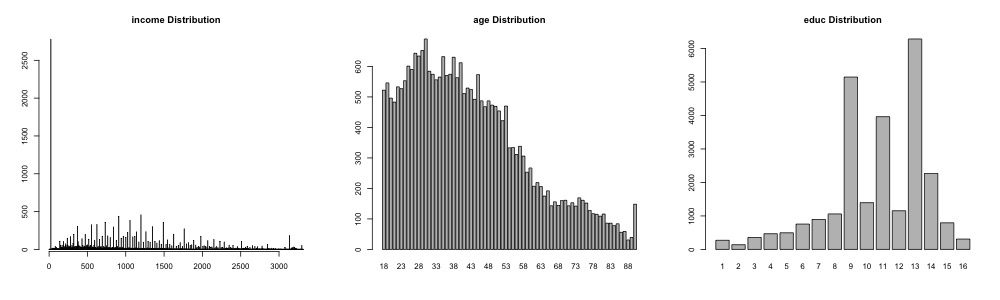
\includegraphics[width=\textwidth]{figs/exploredist}
\end{center}

The goal now is to quantify exactly how identifiable each variable is. Estimates for the probability of collision (of another individual having the exact same value) for each variable based on the largest bin (i.e. worst case) are made below. Actual probabilities for collision can also be calculated by the following formula:
\[p_{collision}=p(X_1 = X_2) = \sum\limits_{x} p(X_1 = x)p(X_2=x) = \sum\limits_x \left(\dfrac{\text{count}(x)}{25766}\right)^2\]
where $x$ is to take on all possible values for that variable.

\texttt{income} is the most identifiable variable but also raises an issue when examining the distribution histogram: a large number of individuals have zero income, and are therefore substantially more difficult to uniquely identify. Apart from this unique case, though, no bin has more than 500 individuals, which corresponds to approximately 500/25766 $\approx$ 2\% of collision with another individual (actual: {0.01555964}). \texttt{age} is distributed a lot better, with the worst case bin having no more than 800 individuals with the same age. When considering the overall size of 25766, that means that there is \emph{at most} a 800/25766 $\approx$ 3\% chance of having the same age as a randomly chosen person in the dataset (actual: {0.01831928}). Lastly, for \texttt{educ}, with up to 6500 in the same bin, the probability of having the same education level as someone else would be 6500/25766 $\approx$ 25\% (actual: {0.1416453}).

Percentage estimates where given above to provide intuition and also as a sanity check, but the actual values calculated will be the ones used from here on.

When taking these three variables together, the probability of the collision is the intersection of all three variables colliding, which is the product of the three probabilities. This gives an overall probability of colliding to be $0.01555964 \times 0.01831928 \times 0.1416453 \approx \textbf{0.00004} = p_{collision}$.

Now, the geographic identifier of PUMA regions needs to be taken into account. Here is a summary of counts for each PUMA region.
\begin{center}
\begin{tabular}{|c|ccccccc|}
\hline
\textbf{PUMA} & 1101 & 1102 & 1103 & 1104 & 1105 & 1106 & 1107\\\hline
\textbf{Count} & 3215 & 5736 & 3728 & 3740 & 3128 & 3236 & 2983\\ \hline
\end{tabular}
\end{center}
These are very roughly equal (i.e. on the same order of magnitude), and these do appear to be 5\% samples (with full populations of ~50000-120000 in each PUMA, which is appropriate). Assume the average PUMA region to therefore be 1/7 of the total dataset: $(1/7) \times 20 \times 25766 = 73617$.

To finally determine the percentage of individuals $p(U)$ within a PUMA that can be uniquely identified by the aforementioned variables, this calculation simply involves the probability of no collision with anyone in that region of size $n$, or:
\[p_{unique} = (1-p_{collision})^{n}\]

In this situation, $p_{collision} = 0.00004, n = 73617$ as calculated above, so:
\[p_{unique} = 0.051183922689063\]

$\therefore$ With the three variables of \texttt{income}, \texttt{age}, \texttt{educ}, approximately $\boxed{5\%}$ of the population within a single PUMA can be identified.

Better reconstruction results can be achieved using more variables. The only remaining variables are binary, which should have roughly 50\% chance of collision (though in actuality it will be higher due to uneven distribution). The lowest probabilities of collision are for \texttt{sex} (0.5014973) and \texttt{married} (0.5046546), two common and relatively evenly distributed binary indicators. When factoring these in, then:
\[p_{collision} = 0.00001 \implies p_{unique} = 0.471312198919265\]
$\therefore$ With the five variables of \texttt{income}, \texttt{age}, \texttt{educ}, \texttt{sex}, \texttt{married}, approximately $\boxed{47\%}$ of the population within a single PUMA can be identified.

While it is more difficult and less likely to orchestrate a reconstruction attack with large numbers of variables, out of interest and completeness, here are some further results. With a sixth variable of \texttt{black}, 68\% of the population can be uniquely identified. With a seventh added variable of \texttt{employed}, 81\% of the population can be uniquely identified. The remaining binary variables have sharply decreasing utility due to their uneven distribution (i.e. almost all individuals have the same value and therefore it is not very helpful in identifying someone).

Finally, some small disclaimers. The results above are all approximate and derived from rough back-of-the-envelope calculations. They are also assuming that these variables are available in external sources for cross-referencing, which may present practical obstacles that may or may not be easy to handle. For example, a specific education encoding is used here. Other government databases may use the same schema, making cross-referencing trivial. Furthermore, knowing an individual's exact education level may also be sufficient to map it to one of the factors in this dataset's \texttt{educ} schema. However, if a different, less granular schema was used (i.e. only 5 levels instead of 16), then cross-referencing may not really be possible. Different levels of granularity would be a particularly common issue for \texttt{income}, with added concerns such as rounding. It may also affect \texttt{age}, though probably to a much lesser extent. Binary variables should otherwise be less problematic in this regard.\\

{\large\textbf{Problem 2}}


{\large\textbf{Problem 3}}


{\large\textbf{Problem 4}}



\begin{lstlisting}

\end{lstlisting}


\end{document}